\section{Introduction}
\label{sec:intro}

\begin{figure}[t]
\centering
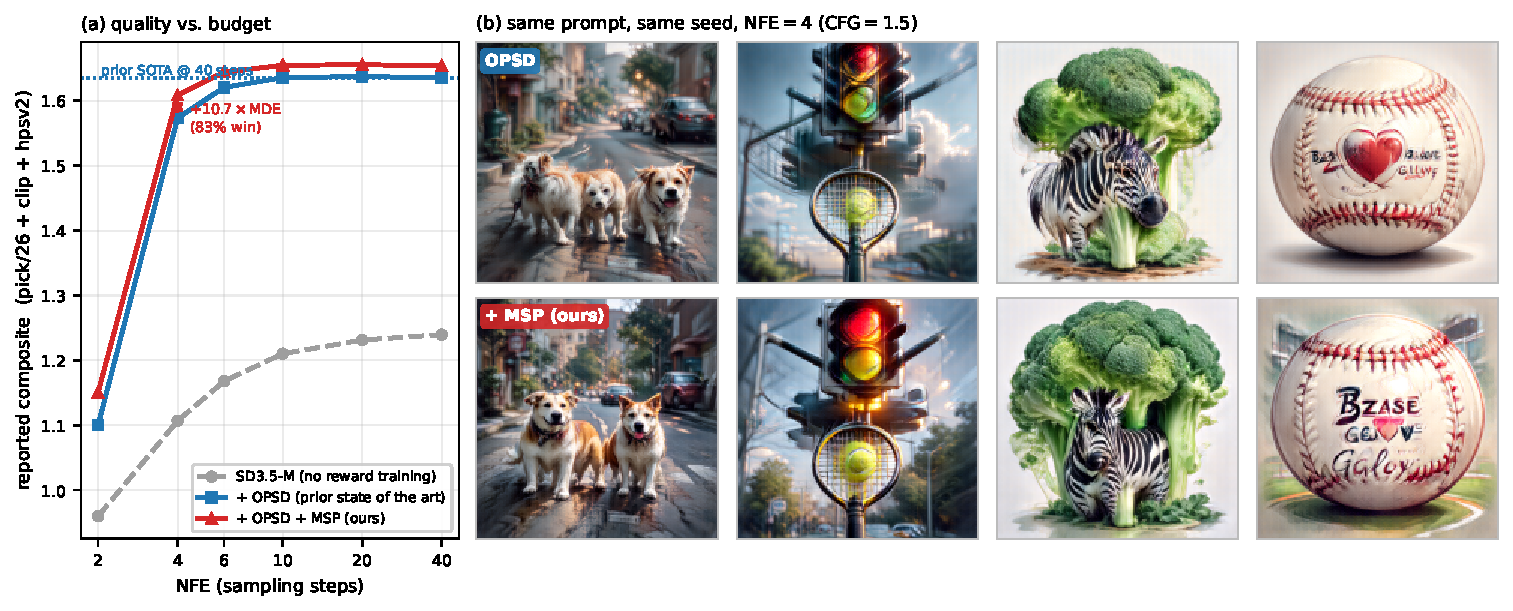
\includegraphics[width=\linewidth]{fig0_teaser.pdf}
\caption{\textbf{Multi-state target propagation (\MSP) makes on-policy reward distillation
budget-robust.} (a) Reported composite versus sampling budget on DrawBench. The prior state
of the art, \opsd, loses most of its advantage once the budget falls below $10$ steps;
propagating the \emph{same} reward-constructed target to higher-noise states of the same
rollout recovers it: on the measured grid it reaches \opsd's $40$-step quality at $6$
sampling steps, where \opsd itself needs $10$.
(b) Same prompts, same seed, $4$ sampling steps, rendered at guidance $1.5$
(App.~\ref{app:protocol}). The four prompts are drawn from the twelve selected in advance by
the rule in App.~\ref{app:qual}, which favours differences checkable by eye -- object counts,
spatial relations and text; all twelve are shown in Fig.~\ref{fig:qual}.}
\label{fig:teaser}
\end{figure}

Aligning a text-to-image diffusion model to a differentiable reward can be cast as
\emph{on-policy self-distillation}: a frozen behavior policy rolls out trajectories, a
reward gradient is converted into a detached target for an intermediate prediction, and
the trainable policy regresses onto that target~\citep{opsd2026,danceopd2026,diffusionopd2026}.
This interface is attractive because the reward and the decoder appear only during target
construction; the fitting step is an ordinary regression and does not retain the reward
graph.

Every method in this family must answer a question that, to our knowledge, has never been
studied: \textbf{at which noise level should the target be built and the loss applied?}
The strongest current method, \opsd, selects a single \emph{low-noise} query
($\sigma^\star\!=\!0.278$, the second-to-last non-degenerate state of a $10$-step
schedule) and applies its loss only there. The choice is defensible -- we confirm in
Sec.~\ref{sec:analysis} that this is where a unit of target displacement buys the most
reward -- but it is made with a single sampling budget in mind.

The consequence shows up as a gap between what a reward-distilled model produces at its
training budget and at a short one, and that gap is \emph{not} a symptom of undertraining.
Trained to the published $300$ updates rather than $100$, the canonical procedure's
$40$-step-versus-$4$-step gap \emph{widens} --- from $19.1$ to $22.3$ MDE on DrawBench and
from $17.1$ to $22.7$ on the held-out prompt set --- because extra budget improves the
full-budget sample faster than the short one. Propagating the target, at the same $100$
updates, moves the gap the other way, to $13.7$ and $12.4$. Training longer aggravates the
problem; changing where the target is applied is what relieves it.

\paragraph{This paper.} We treat the placement of the reward target as the object of
study and evaluate three answers under a strictly matched protocol
(same optimizer budget, same hardware, same seeds, per-image paired tests):

\begin{enumerate}[leftmargin=1.6em,itemsep=2pt]
\item[\textbf{(A)}] \textbf{Move the query state.} Raise $\sigma^\star$ from $0.278$ to
$0.465$. This is a one-line configuration change with \emph{zero} additional cost.
\item[\textbf{(B)}] \textbf{Shorten the training rollout} from $10$ to $6$ steps. This is
\emph{cheaper} than the baseline ($0.90\times$) and moves the query state implicitly,
because the query is selected by nearest-$\sigma$ on the schedule.
\item[\textbf{(C)}] \textbf{Propagate the target (ours).} Keep the low-noise query where
it is, and additionally use the \emph{same} detached target as the regression target at
two higher-noise states of the same rollout. This costs $1.21\times$ and, crucially,
requires \emph{no} additional reward evaluation and \emph{no} additional decoding.
\end{enumerate}

\paragraph{Findings.} (i) (A) and (B) are the same mechanism. Their gain-versus-budget
curves coincide to within measurement error on both prompt sets, and both are a
\emph{trade}: $+12.7$ and $+12.3$ MDE at $4$ sampling steps, but $-0.3$ and $-0.1$ MDE at
the full $40$-step budget ($-1.1$ and $-1.0$ on the held-out prompt set). Raising the
query noise level buys few-step quality by giving up full-budget quality.
(ii) Propagation (C) is \emph{not} a trade. It is the only one of the three
interventions that clears our significance threshold in \emph{all four}
prompt-set~$\times$~budget cells. At $40$ steps it still retains $37\%$ of its peak gain on
DrawBench and $20\%$ on the held-out set, whereas (A) and (B) retain nothing at all --
their full-budget gain has gone slightly negative.
(iii) The two compose: (B$+$C) removes (B)'s full-budget loss \emph{and} attains the
largest few-step gains in the study ($+16.23$ and $+15.91$ MDE, win rates $92.7\%$ and
$95.4\%$). Propagation therefore yields a small family of operating points from one
mechanism -- pure (C) when a single model must serve every budget, (B$+$C) when the
deployment budget is a handful of steps.

\paragraph{Contributions.}
\begin{itemize}[leftmargin=1.4em,itemsep=2pt]
\item We identify target \emph{placement} as an unexamined design axis of on-policy reward
distillation, and show that the placement used by the current state of the art is
suboptimal for few-step sampling by a large margin at zero cost (Sec.~\ref{sec:exp:where}).
\item We propose \textbf{multi-state target propagation} (\MSP): reuse one reward-constructed
target as the regression target at several noise levels of the same trajectory. \MSP adds
no reward evaluations and no decodes, and we show that its per-state backward is
mathematically identical to a joint backward while keeping peak memory at the
single-state level (Sec.~\ref{sec:method}).
\item We give a mechanistic account of why moving the query is a trade and propagating is
not, supported by a measured reward-per-displacement exchange rate across noise levels and
by the height each configuration reaches on the training objective itself
(Sec.~\ref{sec:analysis}).
\item We characterise the design space the method opens. The noise level the supervision
set reaches has an \emph{interior} optimum -- stopping lower or reaching higher are both
worse in every cell -- and the gain survives stacking on the strongest baseline in our
study, which rules out the reading that propagation only helps an under-tuned run
(App.~\ref{app:family}, \ref{app:stack}).
\item We \textbf{map the operating range} of the method rather than only its best point.
Three experiments bound it: raising the branch coefficient from the published $0.1$ to
$1.0$ reverses the gain ($+10.70\to-15.40$ MDE at four steps); training to $300$ updates
instead of $100$ removes the forty-step gain in both of two seeds, and in one of them
collapses the four-step gain as well; and the
reward-specific recipes disagree among themselves, from a significant loss to a significant
gain. We report these because they were
pre-registered comparisons, and they delimit where the method applies
(Sec.~\ref{sec:conclusion}, App.~\ref{app:rewardspec}).
\item We build on a reproduction that we verify against the published protocol rather than
assume. At the published $300$-update budget our canonical run matches the reported row on
\emph{all five} evaluators, and the untrained base model matches to within $1.6\%$, which
isolates the evaluation pipeline from any training code
(Sec.~\ref{sec:exp:repro}). We then report all results against a \emph{measured}
canonical-versus-canonical noise floor and a calibrated held-out evaluator, and release the
calibration (App.~\ref{app:floor}, \ref{app:evalcal}). We believe this protocol is of independent use
to the reward-alignment literature, where effect sizes are frequently of the same order as
run-to-run variation.
\end{itemize}
